\section{Practical Constructions of Symmetric-Key Primitives}
\subsection*{Block Cipher}
Definition: Fixed input size strong PRP\\
$F:\{0,1\}^{n} \times \{0,1\}^{\ell}\rightarrow \{0,1\}^{\ell}$
\begin{itemize}
    \item $n$ - key size
    \item $\ell$ - block size
    \item $n$ and $\ell$ are both fixed
    \item Should take (approximately) $2^n$ time to attack
\end{itemize}

Avalanche Effect: Small change in input must affect every bit of output\\

Confusion-Diffusion  Paradigm
\begin{itemize}
    \item Confusion: $F_k(x)=f_1(x_1)||f_2(x_2)||\cdots||f_{16}(x_16)$
    \begin{itemize}
        \item $|x_i|$ = 8 bits
        \item $f_i$ can be a random permutation on 8 bits
        \item Goal: Introduce random local changes
    \end{itemize}
    \item Diffusion: Shuffle the bits using a mixing permutation
    \begin{itemize}
        \item This just moves bits around
        \item Goal: Spread confusion across all 128 bits
    \end{itemize}
    \item  Repeat many times
\end{itemize}

\subsection*{SPN}
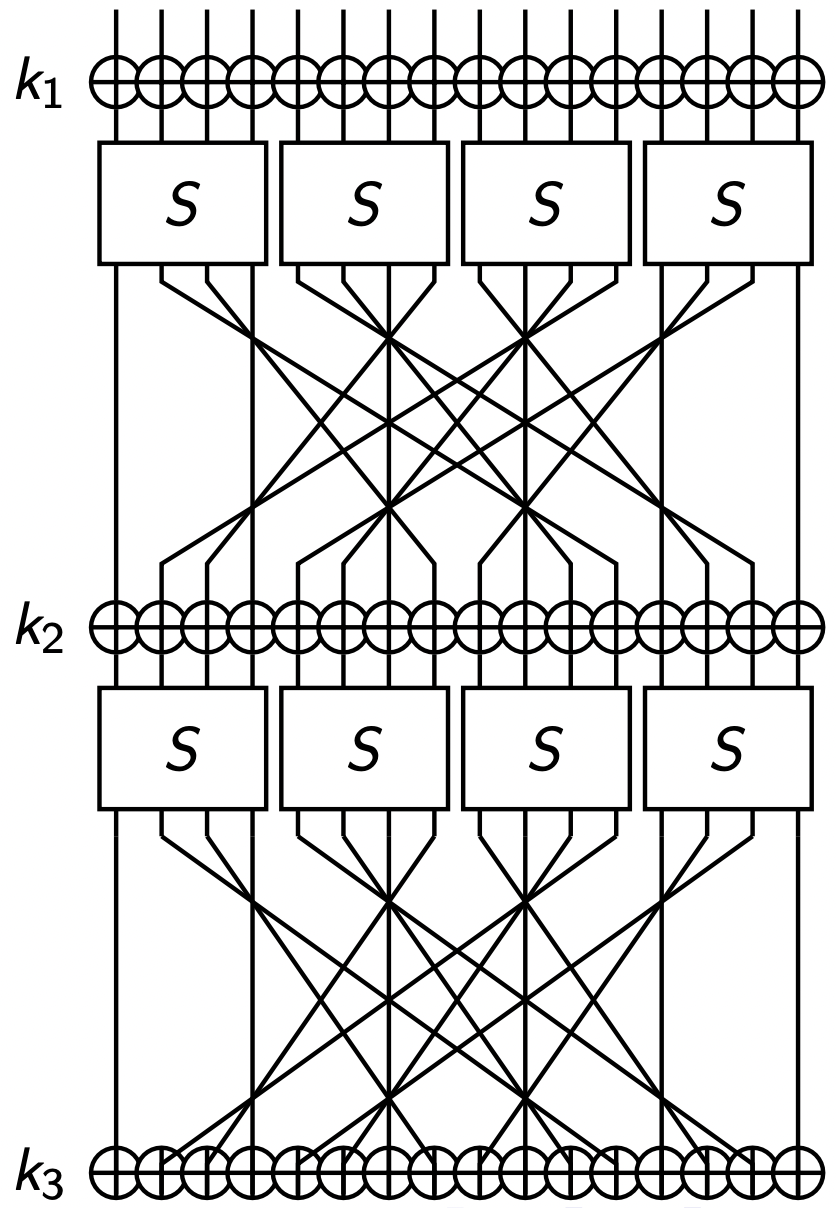
\includegraphics[width=\columnwidth]{SPN.png}\\
Repeat following for many rounds:
\begin{enumerate}
    \item Key mixing: Set $x=x\oplus k_i$
    \item Substitution: $x=S_1(x_1)||\cdots||S_8(x_8)$
    \item Permutation: Permute bits of $x$
\end{enumerate}
